\documentclass[a4paper,11pt,oneside]{article}
\usepackage[ngerman]{babel} % für die deutsche Sprache
\usepackage[T1]{fontenc} % Schriftkodierung (Für Sonderzeichen u.a.)
\usepackage[utf8]{inputenc} % Für die direkte Eingabe von Umlauten im Editor u.a.
\usepackage{fancyhdr} % Für Kopf- und Fußzeilen
\usepackage{lmodern} % Schriftart "Latin Modern"
%\usepackage[normalem]{ulem} % Für das Unterstreichen von Text z.B. mit \uline{}
\usepackage[left=2cm,right=3cm,top=1cm,bottom=1cm,
textheight=245mm,textwidth=160mm,includeheadfoot,headsep=1cm,
footskip=1cm,headheight=14.599pt]{geometry} % Einrichtung der Seite 
\usepackage{setspace} % Paket zum Setzen des Zeilenabstandes
\usepackage{graphicx} % Zum Laden von Graphiken
\usepackage{amsmath}
\usepackage{amsthm}
\usepackage{amsfonts}
\usepackage{hyperref} % Hyperlinks im Inhaltsverzeichnis
\usepackage{pdfpages}
\usepackage{csquotes}
\usepackage{float}

\title{Zusammenfassung zum Capstoneprojekt "MPP-Tracker für einphasigen Wechselrichter
	auf STM32-Basis"}

\author{Jonathan Koeppen, Tobias Magh, Nils Meierhöfer, Moritz Prenzlow, Joshua-Jérôme Reichmann\\ \\ \large{Betreuung durch Prof. C. Dick}}
\date{15.07.2024}

\usepackage[style=numeric,sorting=none]{biblatex} % Stil hier angeben
\addbibresource{Literatur.bib} % .bib Datei hier einbinden

\onehalfspacing

\begin{document}
	\maketitle
	\newpage
	\pagestyle{fancy}
	\tableofcontents

\section{Einleitung}
Dieses Projekt beschäftigt sich mit der Modellierung eines einphasigen PV-Wechselrichters mit Maximum Power Point Tracking (MPPT), der
zum Testen von PV-Modulen eingesetzt wird. Die Implementierung erfolgt in der Software PLECS. Schwerpunkte sind zum einen die
Modellierung des PV-Moduls in Abhängigkeit von Temperatur und Lichtintensität sowie die Implementierung eines Algorithmus für das MPPT
Nachführung. Des Weiteren werden die Detektion eines Lastabwurfs, eine intelligente Abschaltung sowie eine Startroutine untersucht. Darauf
aufbauend soll die implementierte Codegenerierung für einen STM32 aus PLECS heraus durchgeführt und getestet sowie die weitere technisch
mögliche Umsetzung untersucht werden.
\\
\section{Genereller Aufbau}
Die Schaltungstopologie basiert auf einem klassischen einphasigen Wechselrichter. Als Eingang dient ein PV-Modulstrang mit großem DC-Link-Kondensator und Entladewiderstand. Der Wechselrichter ist als H-Brücke ausgeführt. Das AC-Signal wird mit einem Tiefpassfilter geglättet. Die Last wird über einen Transformator als galvanisch getrennter Ausgang angeschlossen. Ein STM32-Mikrocontroller steuert und regelt den Wechselrichter, indem er Schaltsignale aus einer Sinus-PWM an die Leistungshalbleiter sendet. Ein MPP-Tracker stellt dabei den Modulationsgrad für die Sinus-PWM resultierend aus der Eingangsgröße des Tiefpasskondensatorstroms bereit.

\begin{figure}[H]
	\centering
	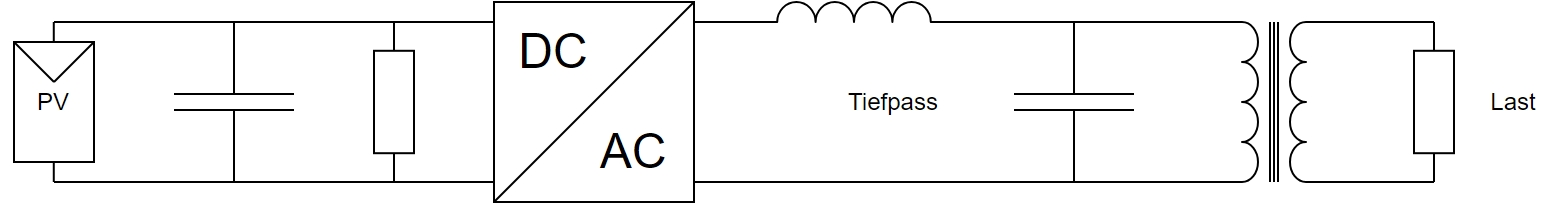
\includegraphics[width=0.8\textwidth]{Aufbau.jpeg}
	\caption{Übersicht der Schaltung}
\end{figure}

\section{Parametrierung}
Die Analyse und Visualisierung der Ergebnisse erfolgt durch die Generierung und Auswertung von CSV-Dateien, die eine strukturierte Darstellung der Daten ermöglichen. Ein PLECS-Simulationsskript wird verwendet, um einen mehrdimensionalen Parameter-Sweep durchzuführen, der verschiedene Kombinationen von Eingabeparametern systematisch untersucht. Parallel dazu wurde eine Parametrisierungsschnittstelle aufgebaut, die eine rudimentäre Eingabe und Anpassung der Parameter erlaubt. Das primäre Ziel dieser Methodik ist die Ermittlung eines optimalen Eingabevektors, der ein vorgegebenes Kriterium bestmöglich erfüllt. Verschiedene Kriterien konnte so getestet werden.\\
Hauptsächlich wurde jedoch getestet, in wie weit es zu Oszillationen innerhalb unseres LC-Tiefpassfiltergliedes kommt, wenn z.B. die Last plötzlich entfernt oder Kurzgeschlossen wird. Zudem interessierte uns, welche Auswirkungen eine Veränderung der PV-Leistung auf die Schaltung haben könnte.\\ Folgende Erkenntnis lässt sich festhalten: Durch Verwenden einer Schaltfrequenz von 48 kHZ und einer Netzfrequenz von 500 Hz, erreichen wir eine ausreichende Distanz zur LC-Resonanzfrequenz von ~ 6 kHz.
Abschalteinrichtungen für z.B. den Kurzschlussfall wurden erprobt, aufgrund der Komplexität welche die Schaltung dann erreichte, wurde für den Rahmen des Capstone-Projekts an dieser Stelle jedoch ein Schlussstrich gezogen.
\\Für weitere Informationen ist im Unterordner Automatisiert\_Testen nachzuschauen.

\begin{figure}[H]
	\centering
	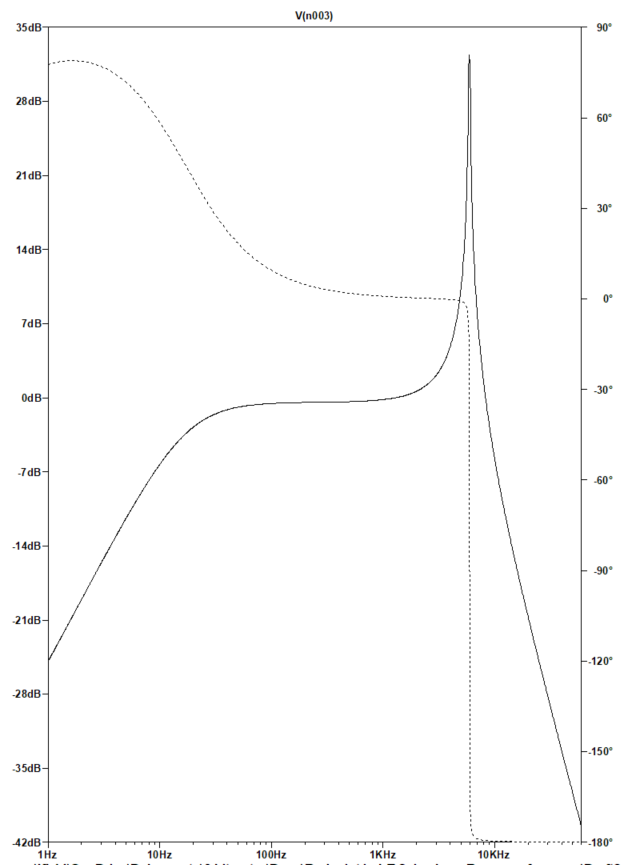
\includegraphics[width=0.8\textwidth]{Bodeplot R fullspec.png}
	\caption{LT-Spice Ausgabe zur Resonanz des LC-Tiefpasses}
\end{figure}

\section{Modellierung einer Lookup-Table}

Um ein beliebiges PV-Modul in PLECS nachzubilden, wird ein Subsystem verwendet, dessen Kernelement eine 3D-Lookup-Tabelle ist, welche eine ideale Stromquelle steuert. Wie eine solche LUT für beliebige PV-Module erstellt und in PLECS eingebunden werden kann, ist in den angehängten Dokumenten beschrieben. Eingangsgrößen des Systems sind die Temperatur und die Sonneneinstrahlung. 
Innerhalb des Subsystems werden die Spannung und der Strom an den Ausgangsklemmen gemessen. Die Strommessung dient allein der Berechnung der Ausgangsleistung, welche durch eine Probe abgelesen werden kann. 
Der Block ist so aufgebaut, dass mehrere PV-Panele in Reihe geschaltet werden können. Aus diesem Grund ist es notwendig, die gemessene Spannung durch die Anzahl der Panele zu teilen, bevor sie als Eingangsgröße der 3D-LUT verwendet werden kann. Die Anzahl der PV-Module wird in der Variable „pv\_strings“ unter den „Simulation Parameters“ initialisiert und in den Blockparametern dem Subsystem übergeben. Bei der Berechnung der LUT kann die Anzahl ebenfalls berücksichtigt werden, jedoch muss dann „pv\_strings“ in PLECS mit „1“ initialisiert sein.
Neben den Eigenschaften des Moduls können auch die elektrischen Eigenschaften der verwendeten Anschlussleitungen berücksichtigt werden. Dazu sind ersatzweise eine Spule, ein Kondensator sowie ein Widerstand mit typischen Größen angelegt, welche wiederum abhängig von der Leitungslänge sind. Diese Länge wird ebenfalls in den „Simulation Parameters“ unter „l\_wire“ initialisiert.\\Für weitere Informationen wird an dieser Stelle auf den Unterordner "PV-LUT" verwiesen.

\section{STM32 Einbindung in PLECS}
Mit der STM32 Plecs-Library ist eine schnelle Adaption von existierenden Simulationen auf reale Hardware möglich. Ein- und Ausgänge des uCs werden durch Blöcke in der Simulation definiert. Die Codegenerierung und Kompilierung findet dann direkt in Plecs statt. Während das Programm auf der Hardware ausgeführt wird, ist ein Betrachten und Setzen von Größen in der bestehenden Simulationsumgebung möglich. 
In diesem Projekt wurde versucht, den STM als "Hardware in the Loop" (HIL) zu betreiben. HIL bedeutet ein Ausführen des Codes auf der eigentlichen Hardware während der Leistungsteil simuliert wird. Für einfache Schaltungen ohne Induktivitäten, Kapazitäten Dioden war der Versuch erfolgreich. Da die Werte der simulierten Ein- und Ausgänge des uCs jedoch nicht in Echtzeit und zu langsam übertragen werden, sind Simulationen komplizierterer Schaltungen nicht möglich. Hierfür muss auf für diese Anwendung entwickelte Hardware zurückgegriffen werden. Es wurde jedoch festgestellt, dass die Anpassung der Simulation des Gleichrichters an den STM sehr einfach ist und mit vorhandener Hardware ein Testen und Debuggen gut möglich wäre. Da Plecs den generierten Code zur Verfügung stellt, könnte dieser auch als Basis für eine von Plecs unabhängige Programmierung verwendet werden.\\Für weitere Informationen wird an dieser Stelle auf den Unterordner STM32 verwiesen.

\begin{figure}[H]
	\centering
	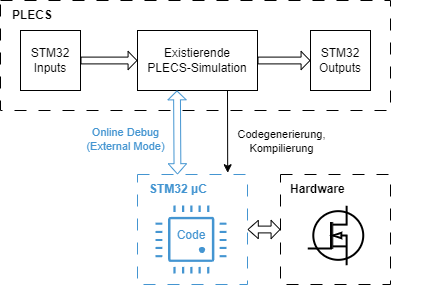
\includegraphics[width=0.8\textwidth]{draft_poster_STM32.drawio.png}
	\caption{Übersicht Anbindung des STM32 an Plecs}
\end{figure}

	\newpage
	\printbibliography
\end{document}